\documentclass[twoside]{book}

% Packages required by doxygen
\usepackage{fixltx2e}
\usepackage{calc}
\usepackage{doxygen}
\usepackage[export]{adjustbox} % also loads graphicx
\usepackage{graphicx}
\usepackage[utf8]{inputenc}
\usepackage{makeidx}
\usepackage{multicol}
\usepackage{multirow}
\PassOptionsToPackage{warn}{textcomp}
\usepackage{textcomp}
\usepackage[nointegrals]{wasysym}
\usepackage[table]{xcolor}

% Font selection
\usepackage[T1]{fontenc}
\usepackage[scaled=.90]{helvet}
\usepackage{courier}
\usepackage{amssymb}
\usepackage{sectsty}
\renewcommand{\familydefault}{\sfdefault}
\allsectionsfont{%
  \fontseries{bc}\selectfont%
  \color{darkgray}%
}
\renewcommand{\DoxyLabelFont}{%
  \fontseries{bc}\selectfont%
  \color{darkgray}%
}
\newcommand{\+}{\discretionary{\mbox{\scriptsize$\hookleftarrow$}}{}{}}

% Page & text layout
\usepackage{geometry}
\geometry{%
  a4paper,%
  top=2.5cm,%
  bottom=2.5cm,%
  left=2.5cm,%
  right=2.5cm%
}
\tolerance=750
\hfuzz=15pt
\hbadness=750
\setlength{\emergencystretch}{15pt}
\setlength{\parindent}{0cm}
\setlength{\parskip}{3ex plus 2ex minus 2ex}
\makeatletter
\renewcommand{\paragraph}{%
  \@startsection{paragraph}{4}{0ex}{-1.0ex}{1.0ex}{%
    \normalfont\normalsize\bfseries\SS@parafont%
  }%
}
\renewcommand{\subparagraph}{%
  \@startsection{subparagraph}{5}{0ex}{-1.0ex}{1.0ex}{%
    \normalfont\normalsize\bfseries\SS@subparafont%
  }%
}
\makeatother

% Headers & footers
\usepackage{fancyhdr}
\pagestyle{fancyplain}
\fancyhead[LE]{\fancyplain{}{\bfseries\thepage}}
\fancyhead[CE]{\fancyplain{}{}}
\fancyhead[RE]{\fancyplain{}{\bfseries\leftmark}}
\fancyhead[LO]{\fancyplain{}{\bfseries\rightmark}}
\fancyhead[CO]{\fancyplain{}{}}
\fancyhead[RO]{\fancyplain{}{\bfseries\thepage}}
\fancyfoot[LE]{\fancyplain{}{}}
\fancyfoot[CE]{\fancyplain{}{}}
\fancyfoot[RE]{\fancyplain{}{\bfseries\scriptsize Generated by Doxygen }}
\fancyfoot[LO]{\fancyplain{}{\bfseries\scriptsize Generated by Doxygen }}
\fancyfoot[CO]{\fancyplain{}{}}
\fancyfoot[RO]{\fancyplain{}{}}
\renewcommand{\footrulewidth}{0.4pt}
\renewcommand{\chaptermark}[1]{%
  \markboth{#1}{}%
}
\renewcommand{\sectionmark}[1]{%
  \markright{\thesection\ #1}%
}

% Indices & bibliography
\usepackage{natbib}
\usepackage[titles]{tocloft}
\setcounter{tocdepth}{3}
\setcounter{secnumdepth}{5}
\makeindex

% Hyperlinks (required, but should be loaded last)
\usepackage{ifpdf}
\ifpdf
  \usepackage[pdftex,pagebackref=true]{hyperref}
\else
  \usepackage[ps2pdf,pagebackref=true]{hyperref}
\fi
\hypersetup{%
  colorlinks=true,%
  linkcolor=blue,%
  citecolor=blue,%
  unicode%
}

% Custom commands
\newcommand{\clearemptydoublepage}{%
  \newpage{\pagestyle{empty}\cleardoublepage}%
}

\usepackage{caption}
\captionsetup{labelsep=space,justification=centering,font={bf},singlelinecheck=off,skip=4pt,position=top}

%===== C O N T E N T S =====

\begin{document}

% Titlepage & ToC
\hypersetup{pageanchor=false,
             bookmarksnumbered=true,
             pdfencoding=unicode
            }
\pagenumbering{alph}
\begin{titlepage}
\vspace*{7cm}
\begin{center}%
{\Large P\+R\+O\+J\+E\+CT T\+E\+T\+R\+IS }\\
\vspace*{1cm}
{\large Generated by Doxygen 1.8.12}\\
\end{center}
\end{titlepage}
\clearemptydoublepage
\pagenumbering{roman}
\tableofcontents
\clearemptydoublepage
\pagenumbering{arabic}
\hypersetup{pageanchor=true}

%--- Begin generated contents ---
\chapter{Main Page}
\label{index}\hypertarget{index}{}This is Team Tetra\textquotesingle{}s (Group 11) final project. It is a redevelopment of the classic game Tetris. 
\chapter{Hierarchical Index}
\section{Class Hierarchy}
This inheritance list is sorted roughly, but not completely, alphabetically\+:\begin{DoxyCompactList}
\item \contentsline{section}{Project\+Tetris.\+Group11.\+Model.\+Piece}{\pageref{class_project_tetris_1_1_group11_1_1_model_1_1_piece}}{}
\item \contentsline{section}{Project\+Tetris.\+Group11.\+Project\+Tetris}{\pageref{class_project_tetris_1_1_group11_1_1_project_tetris}}{}
\item \contentsline{section}{Project\+Tetris.\+Group11.\+Controller.\+Tetris\+Controller}{\pageref{class_project_tetris_1_1_group11_1_1_controller_1_1_tetris_controller}}{}
\item \contentsline{section}{Project\+Tetris.\+Group11.\+Model.\+Well}{\pageref{class_project_tetris_1_1_group11_1_1_model_1_1_well}}{}
\item J\+Frame\begin{DoxyCompactList}
\item \contentsline{section}{Project\+Tetris.\+Group11.\+View.\+Painter}{\pageref{class_project_tetris_1_1_group11_1_1_view_1_1_painter}}{}
\end{DoxyCompactList}
\end{DoxyCompactList}

\chapter{Class Index}
\section{Class List}
Here are the classes, structs, unions and interfaces with brief descriptions\+:\begin{DoxyCompactList}
\item\contentsline{section}{{\bf net.\+tetris.\+controller.\+Game\+Engine} }{\pageref{classnet_1_1tetris_1_1controller_1_1_game_engine}}{}
\item\contentsline{section}{{\bf net.\+tetris.\+model.\+ID} }{\pageref{enumnet_1_1tetris_1_1model_1_1_i_d}}{}
\item\contentsline{section}{{\bf net.\+tetris.\+view.\+Painter} }{\pageref{classnet_1_1tetris_1_1view_1_1_painter}}{}
\item\contentsline{section}{{\bf net.\+tetris.\+model.\+Piece} }{\pageref{classnet_1_1tetris_1_1model_1_1_piece}}{}
\item\contentsline{section}{{\bf net.\+tetris.\+model.\+Tetramino} }{\pageref{classnet_1_1tetris_1_1model_1_1_tetramino}}{}
\item\contentsline{section}{{\bf net.\+tetris.\+model.\+Well} }{\pageref{classnet_1_1tetris_1_1model_1_1_well}}{}
\end{DoxyCompactList}

\chapter{Class Documentation}
\hypertarget{class_project_tetris_1_1_group11_1_1_view_1_1_painter}{}\section{Project\+Tetris.\+Group11.\+View.\+Painter Class Reference}
\label{class_project_tetris_1_1_group11_1_1_view_1_1_painter}\index{Project\+Tetris.\+Group11.\+View.\+Painter@{Project\+Tetris.\+Group11.\+View.\+Painter}}
Inheritance diagram for Project\+Tetris.\+Group11.\+View.\+Painter\+:\begin{figure}[H]
\begin{center}
\leavevmode
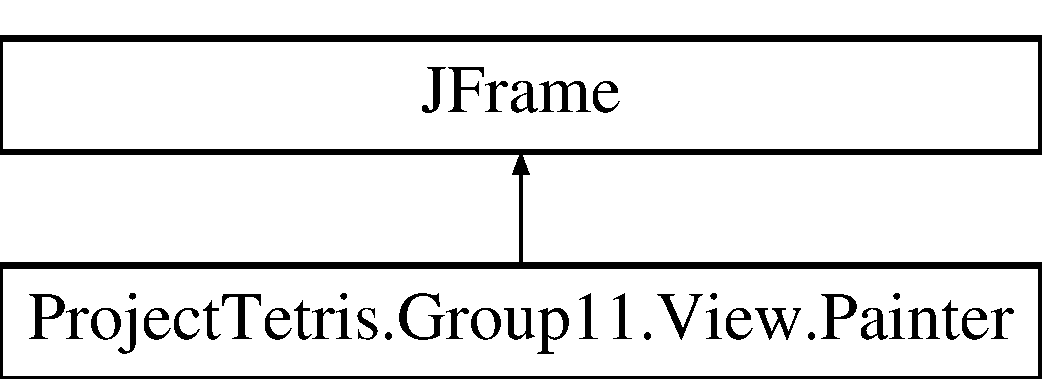
\includegraphics[height=2.000000cm]{class_project_tetris_1_1_group11_1_1_view_1_1_painter}
\end{center}
\end{figure}
\subsection*{Public Member Functions}
\begin{DoxyCompactItemize}
\item 
\hyperlink{class_project_tetris_1_1_group11_1_1_view_1_1_painter_a0a0ad457a5bce0f4292bedd3cefd5201}{Painter} ()
\begin{DoxyCompactList}\small\item\em Constructor for \hyperlink{class_project_tetris_1_1_group11_1_1_view_1_1_painter}{Painter}. \end{DoxyCompactList}\item 
void \hyperlink{class_project_tetris_1_1_group11_1_1_view_1_1_painter_a5df3fdff19e1680167dda4e72f305b93}{set\+Level} (int level)
\begin{DoxyCompactList}\small\item\em This function sets the level of the game. \end{DoxyCompactList}\item 
void \hyperlink{class_project_tetris_1_1_group11_1_1_view_1_1_painter_a53ff8c3c011fba85c87336a10ca9fd47}{set\+Score} (int score)
\begin{DoxyCompactList}\small\item\em This function sets the score of the game. \end{DoxyCompactList}\item 
void \hyperlink{class_project_tetris_1_1_group11_1_1_view_1_1_painter_a9ba776edf8c7be3a910e6b3bace4f1c6}{set\+Well} (\hyperlink{class_project_tetris_1_1_group11_1_1_model_1_1_well}{Well} well)
\begin{DoxyCompactList}\small\item\em This function sets the well to the game. \end{DoxyCompactList}\item 
void \hyperlink{class_project_tetris_1_1_group11_1_1_view_1_1_painter_abf7153f6bf5943456d59db0e677a3920}{set\+Current\+Tetra} (\hyperlink{class_project_tetris_1_1_group11_1_1_model_1_1_piece}{Piece} current\+Tetra)
\begin{DoxyCompactList}\small\item\em This function sets the current piece. \end{DoxyCompactList}\item 
void \hyperlink{class_project_tetris_1_1_group11_1_1_view_1_1_painter_a7094e1d692231ec3e6a3d4d0db2d2860}{set\+Next\+Tetra} (\hyperlink{class_project_tetris_1_1_group11_1_1_model_1_1_piece}{Piece} next\+Tetra)
\begin{DoxyCompactList}\small\item\em This function sets the next piece to be used in the game. \end{DoxyCompactList}\item 
void \hyperlink{class_project_tetris_1_1_group11_1_1_view_1_1_painter_a46e1918a50b4a755e11a69cc723cbea4}{paint} (Graphics g)
\begin{DoxyCompactList}\small\item\em This function draws the total G\+UI. \end{DoxyCompactList}\item 
\hypertarget{class_project_tetris_1_1_group11_1_1_view_1_1_painter_adb62ac5b3377412acc93fb130b4f0572}{}\label{class_project_tetris_1_1_group11_1_1_view_1_1_painter_adb62ac5b3377412acc93fb130b4f0572} 
void \hyperlink{class_project_tetris_1_1_group11_1_1_view_1_1_painter_adb62ac5b3377412acc93fb130b4f0572}{pause\+Message} ()
\begin{DoxyCompactList}\small\item\em This function pauses the game. \end{DoxyCompactList}\item 
\hypertarget{class_project_tetris_1_1_group11_1_1_view_1_1_painter_ad8357a7fc5aaa6aa172f63dd46b58f56}{}\label{class_project_tetris_1_1_group11_1_1_view_1_1_painter_ad8357a7fc5aaa6aa172f63dd46b58f56} 
void \hyperlink{class_project_tetris_1_1_group11_1_1_view_1_1_painter_ad8357a7fc5aaa6aa172f63dd46b58f56}{help\+Message} ()
\begin{DoxyCompactList}\small\item\em This function displays the help dialog which explains how the game works. \end{DoxyCompactList}\item 
\hypertarget{class_project_tetris_1_1_group11_1_1_view_1_1_painter_a5e22d20a037a80e2936a486a66f680d3}{}\label{class_project_tetris_1_1_group11_1_1_view_1_1_painter_a5e22d20a037a80e2936a486a66f680d3} 
void \hyperlink{class_project_tetris_1_1_group11_1_1_view_1_1_painter_a5e22d20a037a80e2936a486a66f680d3}{game\+End} ()
\begin{DoxyCompactList}\small\item\em This function shows the end game dialog. It displays the score and gives the user the option to restart. \end{DoxyCompactList}\item 
void \hyperlink{class_project_tetris_1_1_group11_1_1_view_1_1_painter_a37087ff7a1129d874296ec5bb3ef09d1}{add\+K\+Listener} (Key\+Listener k)
\begin{DoxyCompactList}\small\item\em This function adds a Key\+Listener. \end{DoxyCompactList}\end{DoxyCompactItemize}
\subsection*{Public Attributes}
\begin{DoxyCompactItemize}
\item 
int \hyperlink{class_project_tetris_1_1_group11_1_1_view_1_1_painter_ae72e4845df48232ad82e76f0f2f3fa77}{N\+G\+Input}
\end{DoxyCompactItemize}


\subsection{Constructor \& Destructor Documentation}
\hypertarget{class_project_tetris_1_1_group11_1_1_view_1_1_painter_a0a0ad457a5bce0f4292bedd3cefd5201}{}\label{class_project_tetris_1_1_group11_1_1_view_1_1_painter_a0a0ad457a5bce0f4292bedd3cefd5201} 
\index{Project\+Tetris\+::\+Group11\+::\+View\+::\+Painter@{Project\+Tetris\+::\+Group11\+::\+View\+::\+Painter}!Painter@{Painter}}
\index{Painter@{Painter}!Project\+Tetris\+::\+Group11\+::\+View\+::\+Painter@{Project\+Tetris\+::\+Group11\+::\+View\+::\+Painter}}
\subsubsection{\texorpdfstring{Painter()}{Painter()}}
{\footnotesize\ttfamily Project\+Tetris.\+Group11.\+View.\+Painter.\+Painter (\begin{DoxyParamCaption}{ }\end{DoxyParamCaption})}



Constructor for \hyperlink{class_project_tetris_1_1_group11_1_1_view_1_1_painter}{Painter}. 

Constructor adds the different elements of the G\+UI to the J\+Frame. 

\subsection{Member Function Documentation}
\hypertarget{class_project_tetris_1_1_group11_1_1_view_1_1_painter_a37087ff7a1129d874296ec5bb3ef09d1}{}\label{class_project_tetris_1_1_group11_1_1_view_1_1_painter_a37087ff7a1129d874296ec5bb3ef09d1} 
\index{Project\+Tetris\+::\+Group11\+::\+View\+::\+Painter@{Project\+Tetris\+::\+Group11\+::\+View\+::\+Painter}!add\+K\+Listener@{add\+K\+Listener}}
\index{add\+K\+Listener@{add\+K\+Listener}!Project\+Tetris\+::\+Group11\+::\+View\+::\+Painter@{Project\+Tetris\+::\+Group11\+::\+View\+::\+Painter}}
\subsubsection{\texorpdfstring{add\+K\+Listener()}{addKListener()}}
{\footnotesize\ttfamily void Project\+Tetris.\+Group11.\+View.\+Painter.\+add\+K\+Listener (\begin{DoxyParamCaption}\item[{Key\+Listener}]{k }\end{DoxyParamCaption})}



This function adds a Key\+Listener. 


\begin{DoxyParams}{Parameters}
{\em k} & Key\+Listener to add. \\
\hline
\end{DoxyParams}
\hypertarget{class_project_tetris_1_1_group11_1_1_view_1_1_painter_a46e1918a50b4a755e11a69cc723cbea4}{}\label{class_project_tetris_1_1_group11_1_1_view_1_1_painter_a46e1918a50b4a755e11a69cc723cbea4} 
\index{Project\+Tetris\+::\+Group11\+::\+View\+::\+Painter@{Project\+Tetris\+::\+Group11\+::\+View\+::\+Painter}!paint@{paint}}
\index{paint@{paint}!Project\+Tetris\+::\+Group11\+::\+View\+::\+Painter@{Project\+Tetris\+::\+Group11\+::\+View\+::\+Painter}}
\subsubsection{\texorpdfstring{paint()}{paint()}}
{\footnotesize\ttfamily void Project\+Tetris.\+Group11.\+View.\+Painter.\+paint (\begin{DoxyParamCaption}\item[{Graphics}]{g }\end{DoxyParamCaption})}



This function draws the total G\+UI. 


\begin{DoxyParams}{Parameters}
{\em g} & The Graphics object to draw to. \\
\hline
\end{DoxyParams}
\hypertarget{class_project_tetris_1_1_group11_1_1_view_1_1_painter_abf7153f6bf5943456d59db0e677a3920}{}\label{class_project_tetris_1_1_group11_1_1_view_1_1_painter_abf7153f6bf5943456d59db0e677a3920} 
\index{Project\+Tetris\+::\+Group11\+::\+View\+::\+Painter@{Project\+Tetris\+::\+Group11\+::\+View\+::\+Painter}!set\+Current\+Tetra@{set\+Current\+Tetra}}
\index{set\+Current\+Tetra@{set\+Current\+Tetra}!Project\+Tetris\+::\+Group11\+::\+View\+::\+Painter@{Project\+Tetris\+::\+Group11\+::\+View\+::\+Painter}}
\subsubsection{\texorpdfstring{set\+Current\+Tetra()}{setCurrentTetra()}}
{\footnotesize\ttfamily void Project\+Tetris.\+Group11.\+View.\+Painter.\+set\+Current\+Tetra (\begin{DoxyParamCaption}\item[{\hyperlink{class_project_tetris_1_1_group11_1_1_model_1_1_piece}{Piece}}]{current\+Tetra }\end{DoxyParamCaption})}



This function sets the current piece. 


\begin{DoxyParams}{Parameters}
{\em current\+Tetra} & The current piece in the game. \\
\hline
\end{DoxyParams}
\hypertarget{class_project_tetris_1_1_group11_1_1_view_1_1_painter_a5df3fdff19e1680167dda4e72f305b93}{}\label{class_project_tetris_1_1_group11_1_1_view_1_1_painter_a5df3fdff19e1680167dda4e72f305b93} 
\index{Project\+Tetris\+::\+Group11\+::\+View\+::\+Painter@{Project\+Tetris\+::\+Group11\+::\+View\+::\+Painter}!set\+Level@{set\+Level}}
\index{set\+Level@{set\+Level}!Project\+Tetris\+::\+Group11\+::\+View\+::\+Painter@{Project\+Tetris\+::\+Group11\+::\+View\+::\+Painter}}
\subsubsection{\texorpdfstring{set\+Level()}{setLevel()}}
{\footnotesize\ttfamily void Project\+Tetris.\+Group11.\+View.\+Painter.\+set\+Level (\begin{DoxyParamCaption}\item[{int}]{level }\end{DoxyParamCaption})}



This function sets the level of the game. 


\begin{DoxyParams}{Parameters}
{\em level} & Level of the game. \\
\hline
\end{DoxyParams}
\hypertarget{class_project_tetris_1_1_group11_1_1_view_1_1_painter_a7094e1d692231ec3e6a3d4d0db2d2860}{}\label{class_project_tetris_1_1_group11_1_1_view_1_1_painter_a7094e1d692231ec3e6a3d4d0db2d2860} 
\index{Project\+Tetris\+::\+Group11\+::\+View\+::\+Painter@{Project\+Tetris\+::\+Group11\+::\+View\+::\+Painter}!set\+Next\+Tetra@{set\+Next\+Tetra}}
\index{set\+Next\+Tetra@{set\+Next\+Tetra}!Project\+Tetris\+::\+Group11\+::\+View\+::\+Painter@{Project\+Tetris\+::\+Group11\+::\+View\+::\+Painter}}
\subsubsection{\texorpdfstring{set\+Next\+Tetra()}{setNextTetra()}}
{\footnotesize\ttfamily void Project\+Tetris.\+Group11.\+View.\+Painter.\+set\+Next\+Tetra (\begin{DoxyParamCaption}\item[{\hyperlink{class_project_tetris_1_1_group11_1_1_model_1_1_piece}{Piece}}]{next\+Tetra }\end{DoxyParamCaption})}



This function sets the next piece to be used in the game. 


\begin{DoxyParams}{Parameters}
{\em next\+Tetra} & The next piece. \\
\hline
\end{DoxyParams}
\hypertarget{class_project_tetris_1_1_group11_1_1_view_1_1_painter_a53ff8c3c011fba85c87336a10ca9fd47}{}\label{class_project_tetris_1_1_group11_1_1_view_1_1_painter_a53ff8c3c011fba85c87336a10ca9fd47} 
\index{Project\+Tetris\+::\+Group11\+::\+View\+::\+Painter@{Project\+Tetris\+::\+Group11\+::\+View\+::\+Painter}!set\+Score@{set\+Score}}
\index{set\+Score@{set\+Score}!Project\+Tetris\+::\+Group11\+::\+View\+::\+Painter@{Project\+Tetris\+::\+Group11\+::\+View\+::\+Painter}}
\subsubsection{\texorpdfstring{set\+Score()}{setScore()}}
{\footnotesize\ttfamily void Project\+Tetris.\+Group11.\+View.\+Painter.\+set\+Score (\begin{DoxyParamCaption}\item[{int}]{score }\end{DoxyParamCaption})}



This function sets the score of the game. 


\begin{DoxyParams}{Parameters}
{\em score} & Score of the current game. \\
\hline
\end{DoxyParams}
\hypertarget{class_project_tetris_1_1_group11_1_1_view_1_1_painter_a9ba776edf8c7be3a910e6b3bace4f1c6}{}\label{class_project_tetris_1_1_group11_1_1_view_1_1_painter_a9ba776edf8c7be3a910e6b3bace4f1c6} 
\index{Project\+Tetris\+::\+Group11\+::\+View\+::\+Painter@{Project\+Tetris\+::\+Group11\+::\+View\+::\+Painter}!set\+Well@{set\+Well}}
\index{set\+Well@{set\+Well}!Project\+Tetris\+::\+Group11\+::\+View\+::\+Painter@{Project\+Tetris\+::\+Group11\+::\+View\+::\+Painter}}
\subsubsection{\texorpdfstring{set\+Well()}{setWell()}}
{\footnotesize\ttfamily void Project\+Tetris.\+Group11.\+View.\+Painter.\+set\+Well (\begin{DoxyParamCaption}\item[{\hyperlink{class_project_tetris_1_1_group11_1_1_model_1_1_well}{Well}}]{well }\end{DoxyParamCaption})}



This function sets the well to the game. 


\begin{DoxyParams}{Parameters}
{\em well} & The Well object to set. \\
\hline
\end{DoxyParams}


\subsection{Member Data Documentation}
\hypertarget{class_project_tetris_1_1_group11_1_1_view_1_1_painter_ae72e4845df48232ad82e76f0f2f3fa77}{}\label{class_project_tetris_1_1_group11_1_1_view_1_1_painter_ae72e4845df48232ad82e76f0f2f3fa77} 
\index{Project\+Tetris\+::\+Group11\+::\+View\+::\+Painter@{Project\+Tetris\+::\+Group11\+::\+View\+::\+Painter}!N\+G\+Input@{N\+G\+Input}}
\index{N\+G\+Input@{N\+G\+Input}!Project\+Tetris\+::\+Group11\+::\+View\+::\+Painter@{Project\+Tetris\+::\+Group11\+::\+View\+::\+Painter}}
\subsubsection{\texorpdfstring{N\+G\+Input}{NGInput}}
{\footnotesize\ttfamily int Project\+Tetris.\+Group11.\+View.\+Painter.\+N\+G\+Input}

a public variable for a new game input. 

The documentation for this class was generated from the following file\+:\begin{DoxyCompactItemize}
\item 
C\+:/\+Users/chang/\+Desktop/3\+X\+A3/3\+X\+A3\+\_\+\+Group11/src/\+Project\+Tetris/\+Group11/\+View/Painter.\+java\end{DoxyCompactItemize}

\hypertarget{class_project_tetris_1_1_group11_1_1_model_1_1_piece}{}\section{Project\+Tetris.\+Group11.\+Model.\+Piece Class Reference}
\label{class_project_tetris_1_1_group11_1_1_model_1_1_piece}\index{Project\+Tetris.\+Group11.\+Model.\+Piece@{Project\+Tetris.\+Group11.\+Model.\+Piece}}
\subsection*{Public Member Functions}
\begin{DoxyCompactItemize}
\item 
\hyperlink{class_project_tetris_1_1_group11_1_1_model_1_1_piece_addee3c9cfed3f3a362cad4e89beaa27c}{Piece} (Point\mbox{[}$\,$\mbox{]}\mbox{[}$\,$\mbox{]} piece\+Coords, int pieceX, int pieceY, Color piece\+Color)
\begin{DoxyCompactList}\small\item\em Constructor for \hyperlink{class_project_tetris_1_1_group11_1_1_model_1_1_piece}{Piece}. \end{DoxyCompactList}\item 
\hypertarget{class_project_tetris_1_1_group11_1_1_model_1_1_piece_ac570b95abe339502c9d576673c734748}{}\label{class_project_tetris_1_1_group11_1_1_model_1_1_piece_ac570b95abe339502c9d576673c734748} 
void \hyperlink{class_project_tetris_1_1_group11_1_1_model_1_1_piece_ac570b95abe339502c9d576673c734748}{piece\+Drop} ()
\begin{DoxyCompactList}\small\item\em This function drops the piece down 1 line. \end{DoxyCompactList}\item 
\hypertarget{class_project_tetris_1_1_group11_1_1_model_1_1_piece_a3829a3fe63042cbd4765e59619a9147a}{}\label{class_project_tetris_1_1_group11_1_1_model_1_1_piece_a3829a3fe63042cbd4765e59619a9147a} 
void \hyperlink{class_project_tetris_1_1_group11_1_1_model_1_1_piece_a3829a3fe63042cbd4765e59619a9147a}{move\+Left} ()
\begin{DoxyCompactList}\small\item\em This function moves the piece left over 1 line. \end{DoxyCompactList}\item 
\hypertarget{class_project_tetris_1_1_group11_1_1_model_1_1_piece_ac2d30f3f8e7bb4f156b590ba41a1c24b}{}\label{class_project_tetris_1_1_group11_1_1_model_1_1_piece_ac2d30f3f8e7bb4f156b590ba41a1c24b} 
void \hyperlink{class_project_tetris_1_1_group11_1_1_model_1_1_piece_ac2d30f3f8e7bb4f156b590ba41a1c24b}{move\+Right} ()
\begin{DoxyCompactList}\small\item\em This function moves the piece right over 1 line. \end{DoxyCompactList}\item 
void \hyperlink{class_project_tetris_1_1_group11_1_1_model_1_1_piece_a49a8a87f2d7265970cda241bb0740106}{rotate\+Left} (int newO)
\begin{DoxyCompactList}\small\item\em This function rotates the piece C\+CW. \end{DoxyCompactList}\item 
void \hyperlink{class_project_tetris_1_1_group11_1_1_model_1_1_piece_a9ec88cace1726a50873efb97a8ec84fb}{rotate\+Right} (int newO)
\begin{DoxyCompactList}\small\item\em This function rotates the piece CW. \end{DoxyCompactList}\item 
Point \mbox{[}$\,$\mbox{]} \hyperlink{class_project_tetris_1_1_group11_1_1_model_1_1_piece_ad8329552a5f8d91046075dca5d8897fd}{get\+Piece\+Coords} (int o)
\begin{DoxyCompactList}\small\item\em This function returns the coordinates of a piece at the given position. \end{DoxyCompactList}\item 
void \hyperlink{class_project_tetris_1_1_group11_1_1_model_1_1_piece_aba9188db14387a600e902dadd2d20332}{set\+Piece\+Coords} (Point\mbox{[}$\,$\mbox{]}\mbox{[}$\,$\mbox{]} piece\+Coords)
\begin{DoxyCompactList}\small\item\em This function sets the coordinates of a piece. \end{DoxyCompactList}\item 
int \hyperlink{class_project_tetris_1_1_group11_1_1_model_1_1_piece_a018dce64b98650107e8871e23dd1e152}{get\+PieceX} ()
\begin{DoxyCompactList}\small\item\em This function returns the X coordinate. \end{DoxyCompactList}\item 
void \hyperlink{class_project_tetris_1_1_group11_1_1_model_1_1_piece_a5ea3a78cfb66a1609cf259f9e624dfcb}{set\+PieceX} (int pieceX)
\begin{DoxyCompactList}\small\item\em This function sets the X coordinate. \end{DoxyCompactList}\item 
int \hyperlink{class_project_tetris_1_1_group11_1_1_model_1_1_piece_a4c4c4dacf31d9824f2a223a722833b55}{get\+PieceY} ()
\begin{DoxyCompactList}\small\item\em This function returns the Y coordinate. \end{DoxyCompactList}\item 
void \hyperlink{class_project_tetris_1_1_group11_1_1_model_1_1_piece_a95bc4289b926d0dbc31cffee2089d464}{set\+PieceY} (int pieceY)
\begin{DoxyCompactList}\small\item\em This function sets the Y coordinate. \end{DoxyCompactList}\item 
int \hyperlink{class_project_tetris_1_1_group11_1_1_model_1_1_piece_aaad692840f784a0a1fd016a64830240e}{get\+Orientation} ()
\begin{DoxyCompactList}\small\item\em This function returns the orientation of the piece. \end{DoxyCompactList}\item 
void \hyperlink{class_project_tetris_1_1_group11_1_1_model_1_1_piece_a84cf70c609e13d3a31f7c3815ddff827}{set\+Orientation} (int orientation)
\begin{DoxyCompactList}\small\item\em This function sets the orientation of a piece. \end{DoxyCompactList}\item 
Color \hyperlink{class_project_tetris_1_1_group11_1_1_model_1_1_piece_a0e992758414c2d119d0501d6a7d2cd0f}{get\+Color} ()
\begin{DoxyCompactList}\small\item\em This function returns the color of the piece. \end{DoxyCompactList}\end{DoxyCompactItemize}


\subsection{Constructor \& Destructor Documentation}
\hypertarget{class_project_tetris_1_1_group11_1_1_model_1_1_piece_addee3c9cfed3f3a362cad4e89beaa27c}{}\label{class_project_tetris_1_1_group11_1_1_model_1_1_piece_addee3c9cfed3f3a362cad4e89beaa27c} 
\index{Project\+Tetris\+::\+Group11\+::\+Model\+::\+Piece@{Project\+Tetris\+::\+Group11\+::\+Model\+::\+Piece}!Piece@{Piece}}
\index{Piece@{Piece}!Project\+Tetris\+::\+Group11\+::\+Model\+::\+Piece@{Project\+Tetris\+::\+Group11\+::\+Model\+::\+Piece}}
\subsubsection{\texorpdfstring{Piece()}{Piece()}}
{\footnotesize\ttfamily Project\+Tetris.\+Group11.\+Model.\+Piece.\+Piece (\begin{DoxyParamCaption}\item[{Point}]{piece\+Coords\mbox{[}$\,$\mbox{]}\mbox{[}$\,$\mbox{]},  }\item[{int}]{pieceX,  }\item[{int}]{pieceY,  }\item[{Color}]{piece\+Color }\end{DoxyParamCaption})}



Constructor for \hyperlink{class_project_tetris_1_1_group11_1_1_model_1_1_piece}{Piece}. 

Constructor creates and sets the coordinates and color of the pieces. 
\begin{DoxyParams}{Parameters}
{\em piece\+Coords} & (x,y) coordinates of the shape of the piece. \\
\hline
{\em pieceX} & X coordinates. \\
\hline
{\em pieceY} & Y coordinates. \\
\hline
{\em piece\+Color} & Color. \\
\hline
\end{DoxyParams}


\subsection{Member Function Documentation}
\hypertarget{class_project_tetris_1_1_group11_1_1_model_1_1_piece_a0e992758414c2d119d0501d6a7d2cd0f}{}\label{class_project_tetris_1_1_group11_1_1_model_1_1_piece_a0e992758414c2d119d0501d6a7d2cd0f} 
\index{Project\+Tetris\+::\+Group11\+::\+Model\+::\+Piece@{Project\+Tetris\+::\+Group11\+::\+Model\+::\+Piece}!get\+Color@{get\+Color}}
\index{get\+Color@{get\+Color}!Project\+Tetris\+::\+Group11\+::\+Model\+::\+Piece@{Project\+Tetris\+::\+Group11\+::\+Model\+::\+Piece}}
\subsubsection{\texorpdfstring{get\+Color()}{getColor()}}
{\footnotesize\ttfamily Color Project\+Tetris.\+Group11.\+Model.\+Piece.\+get\+Color (\begin{DoxyParamCaption}{ }\end{DoxyParamCaption})}



This function returns the color of the piece. 

\begin{DoxyReturn}{Returns}
piece\+Color 
\end{DoxyReturn}
\hypertarget{class_project_tetris_1_1_group11_1_1_model_1_1_piece_aaad692840f784a0a1fd016a64830240e}{}\label{class_project_tetris_1_1_group11_1_1_model_1_1_piece_aaad692840f784a0a1fd016a64830240e} 
\index{Project\+Tetris\+::\+Group11\+::\+Model\+::\+Piece@{Project\+Tetris\+::\+Group11\+::\+Model\+::\+Piece}!get\+Orientation@{get\+Orientation}}
\index{get\+Orientation@{get\+Orientation}!Project\+Tetris\+::\+Group11\+::\+Model\+::\+Piece@{Project\+Tetris\+::\+Group11\+::\+Model\+::\+Piece}}
\subsubsection{\texorpdfstring{get\+Orientation()}{getOrientation()}}
{\footnotesize\ttfamily int Project\+Tetris.\+Group11.\+Model.\+Piece.\+get\+Orientation (\begin{DoxyParamCaption}{ }\end{DoxyParamCaption})}



This function returns the orientation of the piece. 

\begin{DoxyReturn}{Returns}
orientation 
\end{DoxyReturn}
\hypertarget{class_project_tetris_1_1_group11_1_1_model_1_1_piece_ad8329552a5f8d91046075dca5d8897fd}{}\label{class_project_tetris_1_1_group11_1_1_model_1_1_piece_ad8329552a5f8d91046075dca5d8897fd} 
\index{Project\+Tetris\+::\+Group11\+::\+Model\+::\+Piece@{Project\+Tetris\+::\+Group11\+::\+Model\+::\+Piece}!get\+Piece\+Coords@{get\+Piece\+Coords}}
\index{get\+Piece\+Coords@{get\+Piece\+Coords}!Project\+Tetris\+::\+Group11\+::\+Model\+::\+Piece@{Project\+Tetris\+::\+Group11\+::\+Model\+::\+Piece}}
\subsubsection{\texorpdfstring{get\+Piece\+Coords()}{getPieceCoords()}}
{\footnotesize\ttfamily Point \mbox{[}$\,$\mbox{]} Project\+Tetris.\+Group11.\+Model.\+Piece.\+get\+Piece\+Coords (\begin{DoxyParamCaption}\item[{int}]{o }\end{DoxyParamCaption})}



This function returns the coordinates of a piece at the given position. 


\begin{DoxyParams}{Parameters}
{\em o} & Position of piece. \\
\hline
\end{DoxyParams}
\begin{DoxyReturn}{Returns}
piece\+Coords 
\end{DoxyReturn}
\hypertarget{class_project_tetris_1_1_group11_1_1_model_1_1_piece_a018dce64b98650107e8871e23dd1e152}{}\label{class_project_tetris_1_1_group11_1_1_model_1_1_piece_a018dce64b98650107e8871e23dd1e152} 
\index{Project\+Tetris\+::\+Group11\+::\+Model\+::\+Piece@{Project\+Tetris\+::\+Group11\+::\+Model\+::\+Piece}!get\+PieceX@{get\+PieceX}}
\index{get\+PieceX@{get\+PieceX}!Project\+Tetris\+::\+Group11\+::\+Model\+::\+Piece@{Project\+Tetris\+::\+Group11\+::\+Model\+::\+Piece}}
\subsubsection{\texorpdfstring{get\+Piece\+X()}{getPieceX()}}
{\footnotesize\ttfamily int Project\+Tetris.\+Group11.\+Model.\+Piece.\+get\+PieceX (\begin{DoxyParamCaption}{ }\end{DoxyParamCaption})}



This function returns the X coordinate. 

\begin{DoxyReturn}{Returns}
pieceX 
\end{DoxyReturn}
\hypertarget{class_project_tetris_1_1_group11_1_1_model_1_1_piece_a4c4c4dacf31d9824f2a223a722833b55}{}\label{class_project_tetris_1_1_group11_1_1_model_1_1_piece_a4c4c4dacf31d9824f2a223a722833b55} 
\index{Project\+Tetris\+::\+Group11\+::\+Model\+::\+Piece@{Project\+Tetris\+::\+Group11\+::\+Model\+::\+Piece}!get\+PieceY@{get\+PieceY}}
\index{get\+PieceY@{get\+PieceY}!Project\+Tetris\+::\+Group11\+::\+Model\+::\+Piece@{Project\+Tetris\+::\+Group11\+::\+Model\+::\+Piece}}
\subsubsection{\texorpdfstring{get\+Piece\+Y()}{getPieceY()}}
{\footnotesize\ttfamily int Project\+Tetris.\+Group11.\+Model.\+Piece.\+get\+PieceY (\begin{DoxyParamCaption}{ }\end{DoxyParamCaption})}



This function returns the Y coordinate. 

\begin{DoxyReturn}{Returns}
pieceY 
\end{DoxyReturn}
\hypertarget{class_project_tetris_1_1_group11_1_1_model_1_1_piece_a49a8a87f2d7265970cda241bb0740106}{}\label{class_project_tetris_1_1_group11_1_1_model_1_1_piece_a49a8a87f2d7265970cda241bb0740106} 
\index{Project\+Tetris\+::\+Group11\+::\+Model\+::\+Piece@{Project\+Tetris\+::\+Group11\+::\+Model\+::\+Piece}!rotate\+Left@{rotate\+Left}}
\index{rotate\+Left@{rotate\+Left}!Project\+Tetris\+::\+Group11\+::\+Model\+::\+Piece@{Project\+Tetris\+::\+Group11\+::\+Model\+::\+Piece}}
\subsubsection{\texorpdfstring{rotate\+Left()}{rotateLeft()}}
{\footnotesize\ttfamily void Project\+Tetris.\+Group11.\+Model.\+Piece.\+rotate\+Left (\begin{DoxyParamCaption}\item[{int}]{newO }\end{DoxyParamCaption})}



This function rotates the piece C\+CW. 


\begin{DoxyParams}{Parameters}
{\em newO} & new orientation of the piece. \\
\hline
\end{DoxyParams}
\hypertarget{class_project_tetris_1_1_group11_1_1_model_1_1_piece_a9ec88cace1726a50873efb97a8ec84fb}{}\label{class_project_tetris_1_1_group11_1_1_model_1_1_piece_a9ec88cace1726a50873efb97a8ec84fb} 
\index{Project\+Tetris\+::\+Group11\+::\+Model\+::\+Piece@{Project\+Tetris\+::\+Group11\+::\+Model\+::\+Piece}!rotate\+Right@{rotate\+Right}}
\index{rotate\+Right@{rotate\+Right}!Project\+Tetris\+::\+Group11\+::\+Model\+::\+Piece@{Project\+Tetris\+::\+Group11\+::\+Model\+::\+Piece}}
\subsubsection{\texorpdfstring{rotate\+Right()}{rotateRight()}}
{\footnotesize\ttfamily void Project\+Tetris.\+Group11.\+Model.\+Piece.\+rotate\+Right (\begin{DoxyParamCaption}\item[{int}]{newO }\end{DoxyParamCaption})}



This function rotates the piece CW. 


\begin{DoxyParams}{Parameters}
{\em newO} & new orientation of the piece. \\
\hline
\end{DoxyParams}
\hypertarget{class_project_tetris_1_1_group11_1_1_model_1_1_piece_a84cf70c609e13d3a31f7c3815ddff827}{}\label{class_project_tetris_1_1_group11_1_1_model_1_1_piece_a84cf70c609e13d3a31f7c3815ddff827} 
\index{Project\+Tetris\+::\+Group11\+::\+Model\+::\+Piece@{Project\+Tetris\+::\+Group11\+::\+Model\+::\+Piece}!set\+Orientation@{set\+Orientation}}
\index{set\+Orientation@{set\+Orientation}!Project\+Tetris\+::\+Group11\+::\+Model\+::\+Piece@{Project\+Tetris\+::\+Group11\+::\+Model\+::\+Piece}}
\subsubsection{\texorpdfstring{set\+Orientation()}{setOrientation()}}
{\footnotesize\ttfamily void Project\+Tetris.\+Group11.\+Model.\+Piece.\+set\+Orientation (\begin{DoxyParamCaption}\item[{int}]{orientation }\end{DoxyParamCaption})}



This function sets the orientation of a piece. 


\begin{DoxyParams}{Parameters}
{\em orientation} & New orientation for the piece. \\
\hline
\end{DoxyParams}
\hypertarget{class_project_tetris_1_1_group11_1_1_model_1_1_piece_aba9188db14387a600e902dadd2d20332}{}\label{class_project_tetris_1_1_group11_1_1_model_1_1_piece_aba9188db14387a600e902dadd2d20332} 
\index{Project\+Tetris\+::\+Group11\+::\+Model\+::\+Piece@{Project\+Tetris\+::\+Group11\+::\+Model\+::\+Piece}!set\+Piece\+Coords@{set\+Piece\+Coords}}
\index{set\+Piece\+Coords@{set\+Piece\+Coords}!Project\+Tetris\+::\+Group11\+::\+Model\+::\+Piece@{Project\+Tetris\+::\+Group11\+::\+Model\+::\+Piece}}
\subsubsection{\texorpdfstring{set\+Piece\+Coords()}{setPieceCoords()}}
{\footnotesize\ttfamily void Project\+Tetris.\+Group11.\+Model.\+Piece.\+set\+Piece\+Coords (\begin{DoxyParamCaption}\item[{Point}]{piece\+Coords\mbox{[}$\,$\mbox{]}\mbox{[}$\,$\mbox{]} }\end{DoxyParamCaption})}



This function sets the coordinates of a piece. 


\begin{DoxyParams}{Parameters}
{\em piece\+Coords} & coordinates of the new position. \\
\hline
\end{DoxyParams}
\hypertarget{class_project_tetris_1_1_group11_1_1_model_1_1_piece_a5ea3a78cfb66a1609cf259f9e624dfcb}{}\label{class_project_tetris_1_1_group11_1_1_model_1_1_piece_a5ea3a78cfb66a1609cf259f9e624dfcb} 
\index{Project\+Tetris\+::\+Group11\+::\+Model\+::\+Piece@{Project\+Tetris\+::\+Group11\+::\+Model\+::\+Piece}!set\+PieceX@{set\+PieceX}}
\index{set\+PieceX@{set\+PieceX}!Project\+Tetris\+::\+Group11\+::\+Model\+::\+Piece@{Project\+Tetris\+::\+Group11\+::\+Model\+::\+Piece}}
\subsubsection{\texorpdfstring{set\+Piece\+X()}{setPieceX()}}
{\footnotesize\ttfamily void Project\+Tetris.\+Group11.\+Model.\+Piece.\+set\+PieceX (\begin{DoxyParamCaption}\item[{int}]{pieceX }\end{DoxyParamCaption})}



This function sets the X coordinate. 


\begin{DoxyParams}{Parameters}
{\em pieceX} & new X coordinate. \\
\hline
\end{DoxyParams}
\hypertarget{class_project_tetris_1_1_group11_1_1_model_1_1_piece_a95bc4289b926d0dbc31cffee2089d464}{}\label{class_project_tetris_1_1_group11_1_1_model_1_1_piece_a95bc4289b926d0dbc31cffee2089d464} 
\index{Project\+Tetris\+::\+Group11\+::\+Model\+::\+Piece@{Project\+Tetris\+::\+Group11\+::\+Model\+::\+Piece}!set\+PieceY@{set\+PieceY}}
\index{set\+PieceY@{set\+PieceY}!Project\+Tetris\+::\+Group11\+::\+Model\+::\+Piece@{Project\+Tetris\+::\+Group11\+::\+Model\+::\+Piece}}
\subsubsection{\texorpdfstring{set\+Piece\+Y()}{setPieceY()}}
{\footnotesize\ttfamily void Project\+Tetris.\+Group11.\+Model.\+Piece.\+set\+PieceY (\begin{DoxyParamCaption}\item[{int}]{pieceY }\end{DoxyParamCaption})}



This function sets the Y coordinate. 


\begin{DoxyParams}{Parameters}
{\em pieceY} & new Y coordinate. \\
\hline
\end{DoxyParams}


The documentation for this class was generated from the following file\+:\begin{DoxyCompactItemize}
\item 
C\+:/\+Users/chang/\+Desktop/3\+X\+A3/3\+X\+A3\+\_\+\+Group11/src/\+Project\+Tetris/\+Group11/\+Model/Piece.\+java\end{DoxyCompactItemize}

\hypertarget{class_project_tetris_1_1_group11_1_1_project_tetris}{}\section{Project\+Tetris.\+Group11.\+Project\+Tetris Class Reference}
\label{class_project_tetris_1_1_group11_1_1_project_tetris}\index{Project\+Tetris.\+Group11.\+Project\+Tetris@{Project\+Tetris.\+Group11.\+Project\+Tetris}}
\subsection*{Static Public Member Functions}
\begin{DoxyCompactItemize}
\item 
\hypertarget{class_project_tetris_1_1_group11_1_1_project_tetris_a085a414cec5f52b4e6da31d0a97f2b2b}{}\label{class_project_tetris_1_1_group11_1_1_project_tetris_a085a414cec5f52b4e6da31d0a97f2b2b} 
static void \hyperlink{class_project_tetris_1_1_group11_1_1_project_tetris_a085a414cec5f52b4e6da31d0a97f2b2b}{main} (String\mbox{[}$\,$\mbox{]} args)
\begin{DoxyCompactList}\small\item\em Main method. Runs the game by creating the Tetris\+Controller. \end{DoxyCompactList}\end{DoxyCompactItemize}


The documentation for this class was generated from the following file\+:\begin{DoxyCompactItemize}
\item 
C\+:/\+Users/chang/\+Desktop/3\+X\+A3/3\+X\+A3\+\_\+\+Group11/src/\+Project\+Tetris/\+Group11/Project\+Tetris.\+java\end{DoxyCompactItemize}

\hypertarget{class_project_tetris_1_1_group11_1_1_controller_1_1_tetris_controller}{}\section{Project\+Tetris.\+Group11.\+Controller.\+Tetris\+Controller Class Reference}
\label{class_project_tetris_1_1_group11_1_1_controller_1_1_tetris_controller}\index{Project\+Tetris.\+Group11.\+Controller.\+Tetris\+Controller@{Project\+Tetris.\+Group11.\+Controller.\+Tetris\+Controller}}
\subsection*{Classes}
\begin{DoxyCompactItemize}
\item 
class {\bfseries K\+Listener}
\begin{DoxyCompactList}\small\item\em This is an inner class defining Key\+Listener that takes the input from view and processes into game commands. \end{DoxyCompactList}\end{DoxyCompactItemize}
\subsection*{Public Member Functions}
\begin{DoxyCompactItemize}
\item 
\hyperlink{class_project_tetris_1_1_group11_1_1_controller_1_1_tetris_controller_a4559dd5c986c8c0a1dc5e4da406196a0}{Tetris\+Controller} ()
\begin{DoxyCompactList}\small\item\em Constructor for the \hyperlink{class_project_tetris_1_1_group11_1_1_controller_1_1_tetris_controller}{Tetris\+Controller}. \end{DoxyCompactList}\item 
\hypertarget{class_project_tetris_1_1_group11_1_1_controller_1_1_tetris_controller_aedbc64c85a0081d8ec2921f81ef2eaf6}{}\label{class_project_tetris_1_1_group11_1_1_controller_1_1_tetris_controller_aedbc64c85a0081d8ec2921f81ef2eaf6} 
void \hyperlink{class_project_tetris_1_1_group11_1_1_controller_1_1_tetris_controller_aedbc64c85a0081d8ec2921f81ef2eaf6}{new\+Game} ()
\begin{DoxyCompactList}\small\item\em This function starts a new game. It instantiates the well and current piece and contains the game loop. \end{DoxyCompactList}\item 
\hypertarget{class_project_tetris_1_1_group11_1_1_controller_1_1_tetris_controller_a7735345ddbb540a588bc05c4f4efa3a4}{}\label{class_project_tetris_1_1_group11_1_1_controller_1_1_tetris_controller_a7735345ddbb540a588bc05c4f4efa3a4} 
void \hyperlink{class_project_tetris_1_1_group11_1_1_controller_1_1_tetris_controller_a7735345ddbb540a588bc05c4f4efa3a4}{set\+Level} ()
\begin{DoxyCompactList}\small\item\em This function determines the level based on the number of Tetriminos dropped and sets speed accordingly. \end{DoxyCompactList}\item 
\hypertarget{class_project_tetris_1_1_group11_1_1_controller_1_1_tetris_controller_a0ec05f8de4a6b4cebc8e9a1937be786c}{}\label{class_project_tetris_1_1_group11_1_1_controller_1_1_tetris_controller_a0ec05f8de4a6b4cebc8e9a1937be786c} 
void \hyperlink{class_project_tetris_1_1_group11_1_1_controller_1_1_tetris_controller_a0ec05f8de4a6b4cebc8e9a1937be786c}{pause} ()
\begin{DoxyCompactList}\small\item\em This function switches the pause state of the game. \end{DoxyCompactList}\item 
\hypertarget{class_project_tetris_1_1_group11_1_1_controller_1_1_tetris_controller_afaa1a6dbdbcf65b0333ebd2d8c421caa}{}\label{class_project_tetris_1_1_group11_1_1_controller_1_1_tetris_controller_afaa1a6dbdbcf65b0333ebd2d8c421caa} 
void \hyperlink{class_project_tetris_1_1_group11_1_1_controller_1_1_tetris_controller_afaa1a6dbdbcf65b0333ebd2d8c421caa}{help} ()
\begin{DoxyCompactList}\small\item\em This function switches the help state. \end{DoxyCompactList}\item 
\hypertarget{class_project_tetris_1_1_group11_1_1_controller_1_1_tetris_controller_a17f89bae4791e3eded4de8e4fa356772}{}\label{class_project_tetris_1_1_group11_1_1_controller_1_1_tetris_controller_a17f89bae4791e3eded4de8e4fa356772} 
void \hyperlink{class_project_tetris_1_1_group11_1_1_controller_1_1_tetris_controller_a17f89bae4791e3eded4de8e4fa356772}{new\+Tetra\+Gen} ()
\begin{DoxyCompactList}\small\item\em This function generates the new Piece and the next piece to be placed. \end{DoxyCompactList}\item 
boolean \hyperlink{class_project_tetris_1_1_group11_1_1_controller_1_1_tetris_controller_afabce707cf2676db630a3219e818162b}{move\+Possible} (\hyperlink{class_project_tetris_1_1_group11_1_1_model_1_1_piece}{Piece} piece, \hyperlink{class_project_tetris_1_1_group11_1_1_model_1_1_well}{Well} well, int x, int y, int o)
\begin{DoxyCompactList}\small\item\em This function checks collision and determines if future piece location will collide with well. \end{DoxyCompactList}\item 
\hypertarget{class_project_tetris_1_1_group11_1_1_controller_1_1_tetris_controller_a53fd55396019d540acc1d3f6cffd3478}{}\label{class_project_tetris_1_1_group11_1_1_controller_1_1_tetris_controller_a53fd55396019d540acc1d3f6cffd3478} 
void \hyperlink{class_project_tetris_1_1_group11_1_1_controller_1_1_tetris_controller_a53fd55396019d540acc1d3f6cffd3478}{piece\+Drop} ()
\begin{DoxyCompactList}\small\item\em This function drops the current piece down 1 space. \end{DoxyCompactList}\item 
\hypertarget{class_project_tetris_1_1_group11_1_1_controller_1_1_tetris_controller_a3d7ce2d5ac30aef5c409a04dc934d6e0}{}\label{class_project_tetris_1_1_group11_1_1_controller_1_1_tetris_controller_a3d7ce2d5ac30aef5c409a04dc934d6e0} 
void \hyperlink{class_project_tetris_1_1_group11_1_1_controller_1_1_tetris_controller_a3d7ce2d5ac30aef5c409a04dc934d6e0}{move\+Left} ()
\begin{DoxyCompactList}\small\item\em This function translates the piece left 1 space. \end{DoxyCompactList}\item 
\hypertarget{class_project_tetris_1_1_group11_1_1_controller_1_1_tetris_controller_a51d583e56759a19f1fb806f4faa86949}{}\label{class_project_tetris_1_1_group11_1_1_controller_1_1_tetris_controller_a51d583e56759a19f1fb806f4faa86949} 
void \hyperlink{class_project_tetris_1_1_group11_1_1_controller_1_1_tetris_controller_a51d583e56759a19f1fb806f4faa86949}{move\+Right} ()
\begin{DoxyCompactList}\small\item\em This function translates the piece right 1 space. \end{DoxyCompactList}\item 
\hypertarget{class_project_tetris_1_1_group11_1_1_controller_1_1_tetris_controller_a7cdb33ab4ffa50deff495173d99ca8d1}{}\label{class_project_tetris_1_1_group11_1_1_controller_1_1_tetris_controller_a7cdb33ab4ffa50deff495173d99ca8d1} 
void \hyperlink{class_project_tetris_1_1_group11_1_1_controller_1_1_tetris_controller_a7cdb33ab4ffa50deff495173d99ca8d1}{rotate\+Left} ()
\begin{DoxyCompactList}\small\item\em This function rotates the current piece C\+CW. \end{DoxyCompactList}\item 
\hypertarget{class_project_tetris_1_1_group11_1_1_controller_1_1_tetris_controller_a5f6b48a2bbf8b617e801f838d1aa4a48}{}\label{class_project_tetris_1_1_group11_1_1_controller_1_1_tetris_controller_a5f6b48a2bbf8b617e801f838d1aa4a48} 
void \hyperlink{class_project_tetris_1_1_group11_1_1_controller_1_1_tetris_controller_a5f6b48a2bbf8b617e801f838d1aa4a48}{rotate\+Right} ()
\begin{DoxyCompactList}\small\item\em This function rotates the current piece CW. \end{DoxyCompactList}\item 
\hypertarget{class_project_tetris_1_1_group11_1_1_controller_1_1_tetris_controller_a061770a9dd0596e04e14e186cfad2523}{}\label{class_project_tetris_1_1_group11_1_1_controller_1_1_tetris_controller_a061770a9dd0596e04e14e186cfad2523} 
void \hyperlink{class_project_tetris_1_1_group11_1_1_controller_1_1_tetris_controller_a061770a9dd0596e04e14e186cfad2523}{send\+To\+Painter} ()
\begin{DoxyCompactList}\small\item\em This function updates the state of the model in the view. \end{DoxyCompactList}\end{DoxyCompactItemize}


\subsection{Constructor \& Destructor Documentation}
\hypertarget{class_project_tetris_1_1_group11_1_1_controller_1_1_tetris_controller_a4559dd5c986c8c0a1dc5e4da406196a0}{}\label{class_project_tetris_1_1_group11_1_1_controller_1_1_tetris_controller_a4559dd5c986c8c0a1dc5e4da406196a0} 
\index{Project\+Tetris\+::\+Group11\+::\+Controller\+::\+Tetris\+Controller@{Project\+Tetris\+::\+Group11\+::\+Controller\+::\+Tetris\+Controller}!Tetris\+Controller@{Tetris\+Controller}}
\index{Tetris\+Controller@{Tetris\+Controller}!Project\+Tetris\+::\+Group11\+::\+Controller\+::\+Tetris\+Controller@{Project\+Tetris\+::\+Group11\+::\+Controller\+::\+Tetris\+Controller}}
\subsubsection{\texorpdfstring{Tetris\+Controller()}{TetrisController()}}
{\footnotesize\ttfamily Project\+Tetris.\+Group11.\+Controller.\+Tetris\+Controller.\+Tetris\+Controller (\begin{DoxyParamCaption}{ }\end{DoxyParamCaption})}



Constructor for the \hyperlink{class_project_tetris_1_1_group11_1_1_controller_1_1_tetris_controller}{Tetris\+Controller}. 

Constructor creates a new painter and adds the K\+Listener. Also starts a new game. 

\subsection{Member Function Documentation}
\hypertarget{class_project_tetris_1_1_group11_1_1_controller_1_1_tetris_controller_afabce707cf2676db630a3219e818162b}{}\label{class_project_tetris_1_1_group11_1_1_controller_1_1_tetris_controller_afabce707cf2676db630a3219e818162b} 
\index{Project\+Tetris\+::\+Group11\+::\+Controller\+::\+Tetris\+Controller@{Project\+Tetris\+::\+Group11\+::\+Controller\+::\+Tetris\+Controller}!move\+Possible@{move\+Possible}}
\index{move\+Possible@{move\+Possible}!Project\+Tetris\+::\+Group11\+::\+Controller\+::\+Tetris\+Controller@{Project\+Tetris\+::\+Group11\+::\+Controller\+::\+Tetris\+Controller}}
\subsubsection{\texorpdfstring{move\+Possible()}{movePossible()}}
{\footnotesize\ttfamily boolean Project\+Tetris.\+Group11.\+Controller.\+Tetris\+Controller.\+move\+Possible (\begin{DoxyParamCaption}\item[{\hyperlink{class_project_tetris_1_1_group11_1_1_model_1_1_piece}{Piece}}]{piece,  }\item[{\hyperlink{class_project_tetris_1_1_group11_1_1_model_1_1_well}{Well}}]{well,  }\item[{int}]{x,  }\item[{int}]{y,  }\item[{int}]{o }\end{DoxyParamCaption})}



This function checks collision and determines if future piece location will collide with well. 

\begin{DoxyReturn}{Returns}
True if piece can move; False if it collides 
\end{DoxyReturn}


The documentation for this class was generated from the following file\+:\begin{DoxyCompactItemize}
\item 
C\+:/\+Users/chang/\+Desktop/3\+X\+A3/3\+X\+A3\+\_\+\+Group11/src/\+Project\+Tetris/\+Group11/\+Controller/Tetris\+Controller.\+java\end{DoxyCompactItemize}

\hypertarget{class_project_tetris_1_1_group11_1_1_model_1_1_well}{}\section{Project\+Tetris.\+Group11.\+Model.\+Well Class Reference}
\label{class_project_tetris_1_1_group11_1_1_model_1_1_well}\index{Project\+Tetris.\+Group11.\+Model.\+Well@{Project\+Tetris.\+Group11.\+Model.\+Well}}
\subsection*{Public Member Functions}
\begin{DoxyCompactItemize}
\item 
\hyperlink{class_project_tetris_1_1_group11_1_1_model_1_1_well_ad2e8ce275ae537968a865f4bc4353455}{Well} ()
\begin{DoxyCompactList}\small\item\em Constructor for the \hyperlink{class_project_tetris_1_1_group11_1_1_model_1_1_well}{Well}. \end{DoxyCompactList}\item 
void \hyperlink{class_project_tetris_1_1_group11_1_1_model_1_1_well_a2b6fbb33b9636deb0389481b90ad6ac3}{add\+To\+Well} (Point\mbox{[}$\,$\mbox{]} piece\+Coords, int pieceX, int pieceY)
\begin{DoxyCompactList}\small\item\em This function adds a piece to the well. \end{DoxyCompactList}\item 
Array\+List$<$ Point $>$ \hyperlink{class_project_tetris_1_1_group11_1_1_model_1_1_well_a16f565cb48b17ea4df866b05a2ea3b36}{get\+Well\+Coords} ()
\begin{DoxyCompactList}\small\item\em This function returns the coordinates for the well. \end{DoxyCompactList}\item 
void \hyperlink{class_project_tetris_1_1_group11_1_1_model_1_1_well_a0d596baf44d364cba8a4f457d064c8cf}{set\+Well\+Coords} (Array\+List$<$ Point $>$ well\+Coords)
\begin{DoxyCompactList}\small\item\em This function sets the coordinates for the well. \end{DoxyCompactList}\item 
Color \hyperlink{class_project_tetris_1_1_group11_1_1_model_1_1_well_a7f4f1bd6f6f38f6c3178dd86d0f8b7b9}{get\+Border\+Color} ()
\begin{DoxyCompactList}\small\item\em This function returns the color of the border. \end{DoxyCompactList}\item 
Color \hyperlink{class_project_tetris_1_1_group11_1_1_model_1_1_well_a587848104b6b00ef0e953e5d43fd4e62}{get\+Well\+Color} ()
\begin{DoxyCompactList}\small\item\em This function returns the color of the well. \end{DoxyCompactList}\end{DoxyCompactItemize}


\subsection{Constructor \& Destructor Documentation}
\hypertarget{class_project_tetris_1_1_group11_1_1_model_1_1_well_ad2e8ce275ae537968a865f4bc4353455}{}\label{class_project_tetris_1_1_group11_1_1_model_1_1_well_ad2e8ce275ae537968a865f4bc4353455} 
\index{Project\+Tetris\+::\+Group11\+::\+Model\+::\+Well@{Project\+Tetris\+::\+Group11\+::\+Model\+::\+Well}!Well@{Well}}
\index{Well@{Well}!Project\+Tetris\+::\+Group11\+::\+Model\+::\+Well@{Project\+Tetris\+::\+Group11\+::\+Model\+::\+Well}}
\subsubsection{\texorpdfstring{Well()}{Well()}}
{\footnotesize\ttfamily Project\+Tetris.\+Group11.\+Model.\+Well.\+Well (\begin{DoxyParamCaption}{ }\end{DoxyParamCaption})}



Constructor for the \hyperlink{class_project_tetris_1_1_group11_1_1_model_1_1_well}{Well}. 

Constructor creates the well object. 

\subsection{Member Function Documentation}
\hypertarget{class_project_tetris_1_1_group11_1_1_model_1_1_well_a2b6fbb33b9636deb0389481b90ad6ac3}{}\label{class_project_tetris_1_1_group11_1_1_model_1_1_well_a2b6fbb33b9636deb0389481b90ad6ac3} 
\index{Project\+Tetris\+::\+Group11\+::\+Model\+::\+Well@{Project\+Tetris\+::\+Group11\+::\+Model\+::\+Well}!add\+To\+Well@{add\+To\+Well}}
\index{add\+To\+Well@{add\+To\+Well}!Project\+Tetris\+::\+Group11\+::\+Model\+::\+Well@{Project\+Tetris\+::\+Group11\+::\+Model\+::\+Well}}
\subsubsection{\texorpdfstring{add\+To\+Well()}{addToWell()}}
{\footnotesize\ttfamily void Project\+Tetris.\+Group11.\+Model.\+Well.\+add\+To\+Well (\begin{DoxyParamCaption}\item[{Point \mbox{[}$\,$\mbox{]}}]{piece\+Coords,  }\item[{int}]{pieceX,  }\item[{int}]{pieceY }\end{DoxyParamCaption})}



This function adds a piece to the well. 


\begin{DoxyParams}{Parameters}
{\em piece\+Coords} & orientation coordinates of piece. \\
\hline
{\em pieceX} & x coordinate of piece. \\
\hline
{\em pieceY} & y coordinate of piece. \\
\hline
\end{DoxyParams}
\hypertarget{class_project_tetris_1_1_group11_1_1_model_1_1_well_a7f4f1bd6f6f38f6c3178dd86d0f8b7b9}{}\label{class_project_tetris_1_1_group11_1_1_model_1_1_well_a7f4f1bd6f6f38f6c3178dd86d0f8b7b9} 
\index{Project\+Tetris\+::\+Group11\+::\+Model\+::\+Well@{Project\+Tetris\+::\+Group11\+::\+Model\+::\+Well}!get\+Border\+Color@{get\+Border\+Color}}
\index{get\+Border\+Color@{get\+Border\+Color}!Project\+Tetris\+::\+Group11\+::\+Model\+::\+Well@{Project\+Tetris\+::\+Group11\+::\+Model\+::\+Well}}
\subsubsection{\texorpdfstring{get\+Border\+Color()}{getBorderColor()}}
{\footnotesize\ttfamily Color Project\+Tetris.\+Group11.\+Model.\+Well.\+get\+Border\+Color (\begin{DoxyParamCaption}{ }\end{DoxyParamCaption})}



This function returns the color of the border. 

\begin{DoxyReturn}{Returns}
border\+Color 
\end{DoxyReturn}
\hypertarget{class_project_tetris_1_1_group11_1_1_model_1_1_well_a587848104b6b00ef0e953e5d43fd4e62}{}\label{class_project_tetris_1_1_group11_1_1_model_1_1_well_a587848104b6b00ef0e953e5d43fd4e62} 
\index{Project\+Tetris\+::\+Group11\+::\+Model\+::\+Well@{Project\+Tetris\+::\+Group11\+::\+Model\+::\+Well}!get\+Well\+Color@{get\+Well\+Color}}
\index{get\+Well\+Color@{get\+Well\+Color}!Project\+Tetris\+::\+Group11\+::\+Model\+::\+Well@{Project\+Tetris\+::\+Group11\+::\+Model\+::\+Well}}
\subsubsection{\texorpdfstring{get\+Well\+Color()}{getWellColor()}}
{\footnotesize\ttfamily Color Project\+Tetris.\+Group11.\+Model.\+Well.\+get\+Well\+Color (\begin{DoxyParamCaption}{ }\end{DoxyParamCaption})}



This function returns the color of the well. 

\begin{DoxyReturn}{Returns}
well\+Color 
\end{DoxyReturn}
\hypertarget{class_project_tetris_1_1_group11_1_1_model_1_1_well_a16f565cb48b17ea4df866b05a2ea3b36}{}\label{class_project_tetris_1_1_group11_1_1_model_1_1_well_a16f565cb48b17ea4df866b05a2ea3b36} 
\index{Project\+Tetris\+::\+Group11\+::\+Model\+::\+Well@{Project\+Tetris\+::\+Group11\+::\+Model\+::\+Well}!get\+Well\+Coords@{get\+Well\+Coords}}
\index{get\+Well\+Coords@{get\+Well\+Coords}!Project\+Tetris\+::\+Group11\+::\+Model\+::\+Well@{Project\+Tetris\+::\+Group11\+::\+Model\+::\+Well}}
\subsubsection{\texorpdfstring{get\+Well\+Coords()}{getWellCoords()}}
{\footnotesize\ttfamily Array\+List$<$Point$>$ Project\+Tetris.\+Group11.\+Model.\+Well.\+get\+Well\+Coords (\begin{DoxyParamCaption}{ }\end{DoxyParamCaption})}



This function returns the coordinates for the well. 

\begin{DoxyReturn}{Returns}
well\+Coords 
\end{DoxyReturn}
\hypertarget{class_project_tetris_1_1_group11_1_1_model_1_1_well_a0d596baf44d364cba8a4f457d064c8cf}{}\label{class_project_tetris_1_1_group11_1_1_model_1_1_well_a0d596baf44d364cba8a4f457d064c8cf} 
\index{Project\+Tetris\+::\+Group11\+::\+Model\+::\+Well@{Project\+Tetris\+::\+Group11\+::\+Model\+::\+Well}!set\+Well\+Coords@{set\+Well\+Coords}}
\index{set\+Well\+Coords@{set\+Well\+Coords}!Project\+Tetris\+::\+Group11\+::\+Model\+::\+Well@{Project\+Tetris\+::\+Group11\+::\+Model\+::\+Well}}
\subsubsection{\texorpdfstring{set\+Well\+Coords()}{setWellCoords()}}
{\footnotesize\ttfamily void Project\+Tetris.\+Group11.\+Model.\+Well.\+set\+Well\+Coords (\begin{DoxyParamCaption}\item[{Array\+List$<$ Point $>$}]{well\+Coords }\end{DoxyParamCaption})}



This function sets the coordinates for the well. 


\begin{DoxyParams}{Parameters}
{\em well\+Coords} & new coordinates for the well. \\
\hline
\end{DoxyParams}


The documentation for this class was generated from the following file\+:\begin{DoxyCompactItemize}
\item 
C\+:/\+Users/chang/\+Desktop/3\+X\+A3/3\+X\+A3\+\_\+\+Group11/src/\+Project\+Tetris/\+Group11/\+Model/Well.\+java\end{DoxyCompactItemize}

%--- End generated contents ---

% Index
\backmatter
\newpage
\phantomsection
\clearemptydoublepage
\addcontentsline{toc}{chapter}{Index}
\printindex

\end{document}
